\documentclass{beamer}
\usetheme[deutsch]{KIT}

\usepackage[utf8]{inputenc}
\usepackage[T1]{fontenc}
\usepackage{babel}
\usepackage{tikz,calc,ifthen}
\usepackage{mathtools}
\usepackage[normalem]{ulem}
\usepackage{graphicx}

\usetikzlibrary{positioning,calc,arrows,shapes}
\tikzset{
  every node/.style={transform shape},
  auto,
  block/.style={align=center,rectangle,draw,minimum height=20pt,minimum width=30pt},
  >=triangle 60,
  alt/.code args={<#1>#2#3}{%
      \alt<#1>{\pgfkeysalso{#2}}{\pgfkeysalso{#3}}
  },
  beameralert/.style={alt=<#1>{color=green!80!black}{}},
  mythick/.style={line width=1.4pt}
}

\newcommand*{\maxwidthofm}[2]{\maxof{\widthof{$#1$}}{\widthof{$#2$}}}
\newcommand<>*{\robustaltm}[2]{
  \alt#3
  {\mathmakebox[\maxwidthofm{#1}{#2}]{#1}\vphantom{#1#2}}
    {\mathmakebox[\maxwidthofm{#1}{#2}]{#2}\vphantom{#1#2}}
}

\newcommand<>*{\nodealert}[1]{\only#2{\draw[overlay,mythick,color=green!80!black] (#1.north west) rectangle (#1.south east)}}

\title{Invasives Rust}
\author{Hermann Heinz Erich Krumrey}
\subtitle{\insertauthor}
\institute[IPD]{Lehrstuhl Programmierparadigmen, IPD Snelting}
\date{29.10.2013}
\KITtitleimage{images/cover.png}

\begin{document}

\begin{frame}
  \maketitle
\end{frame}

\begin{frame}{Struktur}
\begin{enumerate}
  \item TODO Remove this slide!
  \item Motivation + Beispiel
  \item Invasives Rechnen
  \item SPARC
  \item Rust
  \item Octorust + LoC
  \item Octolib + LoC
  \item Leistungsevaluation
  \item Zusammenfassung
  \item Wichtigste 4 Folien
\end{enumerate}
\end{frame}

\begin{frame}{Motivation}
	Beispiel
	Paralleles Problem.
	Brauchst erst 4 Prozessoren I/O ?
	Dann Sequentiell - Netwerk - Bandbreite == Bottleneck Daten Holen
	Dann 8 weil's schneller gehen muss
\end{frame}

\begin{frame}{Invasives Rechnen}
  \only<1-2>{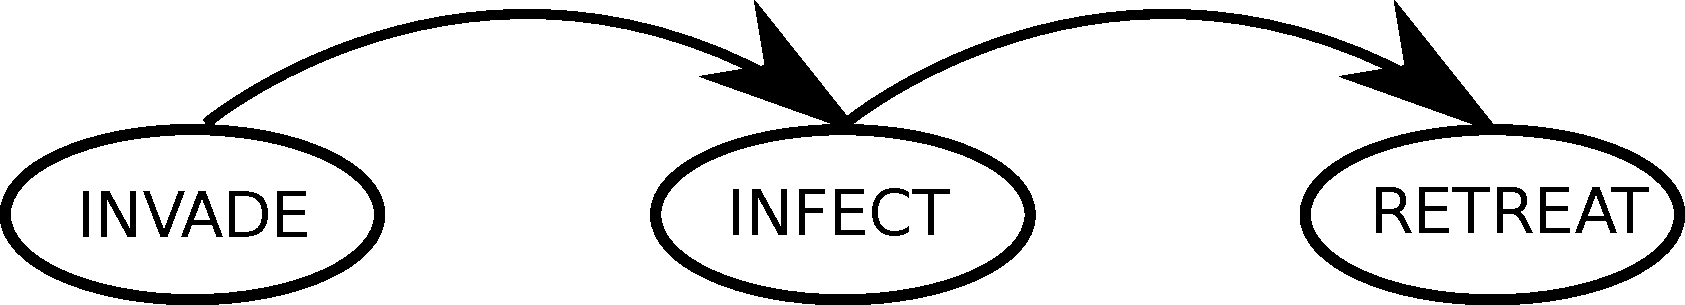
\includegraphics[width=0.4\textwidth]{images/invasiveComputing.pdf}}
  \only<2-3>{
\includegraphics[width=0.4\textwidth]{images/cover.png}}
\end{frame}

\begin{frame}{SPARC LEON}
\end{frame}

\begin{frame}{Rust - Übersicht und Motivation}
\end{frame}

\begin{frame}{Rust - Ownership, Move, Borrow}
\end{frame}

\begin{frame}{Rust - SPARC}
\end{frame}

\begin{frame}{octorust}
	LoC
\end{frame}

\begin{frame}{octolib - Rust Bindings}
	LoC
\end{frame}

\begin{frame}{octolib - Rust Improvements}
	LoC
\end{frame}

\begin{frame}{Evaluation - Laufzeit}
\end{frame}

\begin{frame}{Zusammenfassung und Fazit}
\end{frame}

\begin{frame}{Fragen?}
	4 Wichtigste Folien:
	
	invasive computing
	
	ownership
	
	structs etc
	
	octolib - improvements
\end{frame}

\end{document}
